\section{Correction du code}
\subsection{Gestion du nombre d'arguments}
Dans un premier temps, nous allons mettre en place un système permettant de traiter le cas où le nombre d'arguments n'est pas suffisant. Pour ce faire, nous allons faire un test sur la variable \textit{argc} :
\begin{lstlisting}
/* Checking if we have only two arguments given */
    if (argc == 3)
    {
    ...
    /* code */
    ...
    }else{
	if (argc < 3)
	{
	    /* If there are less than two arguments given, */
	    /* exiting with error code 1 */
	    perror("Too few arguments");
	    return 1;
	}else{
	    /* If there are more than two arguments given, */
	    /* exiting with error code 2 */
	    perror("Too many arguments");
	    return 2;
	}
    }
\end{lstlisting}
Ainsi, si nous exécutons le code en n'ayant pas deux arguments, nous obtiendrons les résultats suivants :
\begin{figure}[H]
 \centering
 \begin{subfigure}[b]{0.9\textwidth}
  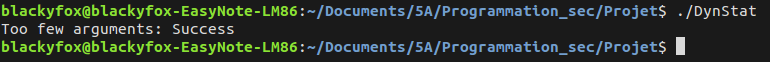
\includegraphics[width=\textwidth]{img/corr1.png}
  \caption{Résultat sans argument}
  \label{img:8.1}
 \end{subfigure}
 ~
 \begin{subfigure}[b]{0.9\textwidth}
  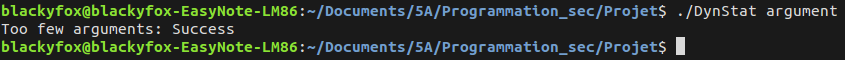
\includegraphics[width=\textwidth]{img/corr2.png}
  \caption{Résultat avec un argument}
  \label{img:8.2}
 \end{subfigure}
 ~
 \begin{subfigure}[b]{0.9\textwidth}
  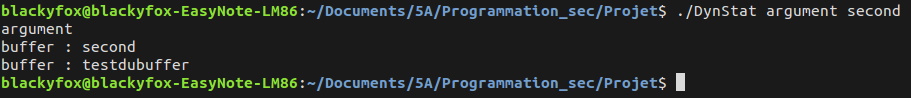
\includegraphics[width=\textwidth]{img/corr3.png}
  \caption{Résultat avec 2 arguments}
  \label{img:8.3}
 \end{subfigure}
 ~
 \begin{subfigure}[b]{0.9\textwidth}
  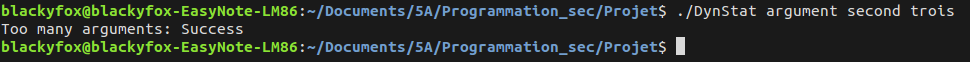
\includegraphics[width=\textwidth]{img/corr4.png}
  \caption{Résultat avec 3 d'arguments ou plus}
  \label{img:8.4}
 \end{subfigure}
 \caption{Résultats en fonction du nombre d'arguments}
\end{figure}

\subsection{Gestion des buffers}

Comme nous avons pu le voir précédemment, nous devons ici récupérer deux chaînes de caractères données en arguments à notre programme. Il est alors intéressant d'utiliser deux buffers pour stocker ces deux variables.\\
Nous allons donc dans un premier temps créer ces variables :
\begin{lstlisting}[language=C]
char* buf1 = NULL;
char* buf2 = NULL;
\end{lstlisting}
Nous allons ensuite allouer dynamiquement l'espace mémoire de ces variables. Nous limiterons leur taille grâce à la variable \textit{size}.\\
Pour ce faire, nous utilisons la fonction \textit{calloc}. Cette fonction est intéressante pour nous car en plus de permettre une allocation dynamique de la mémoire comme la fonction \textit{malloc}, elle va permettre de remplir cet espace mémoire de 0. Ainsi, aucune corruption dues au données présentent à cet espace précédemment ne pourrons interférer avec notre programme.
\begin{lstlisting}[language=C]
buf1 = (char*)calloc(strnlen(argv[1], size)+1, sizeof(char));
buf2 = (char*)calloc(strnlen(argv[2], size)+1, sizeof(char));
\end{lstlisting}
Ainsi, la taille allouée correspond à la taille de l'argument, majorée par la variable \textit{size}\footnote{Ici $\textit{size} = 16$}.\\
Ensuite, nous allons récupérer les chaînes de caractères données en arguments et stocker dans les buffers prévus à cet effet. Pour cela, nous allons utiliser la fonction \textit{snprintf}. Cette dernière va pouvoir nous permettre de copier les contenus d'\textit{argv[1]} et d'\textit{argv[2]} de manière beaucoup contrôlée. En effet, cette fonction va nous permettre de vérifier si la taille des données n'est pas supérieure à la taille du buffer d'arrivée contrairement à la fonction \textit{strcpy}. Cela va ainsi nous permettre de limiter la taille des données traitées afin d'empêcher un \textit{buffer overflow}.\\
La copie se fait alors de la manière suivante :
\begin{lstlisting}[language=C]
if(snprintf(buf1, strnlen(argv[1], size)+1, "%s", argv[1]) < 0){
  perror("Wrinting on variable failed");
  return 5;
}
  if(snprintf(buf2, strnlen(argv[2], size)+1, "%s", argv[2]) < 0){
  perror("Wrinting on variable failed");
  return 6;
}
\end{lstlisting}
De plus nous plaçons cette fonction dans un test conditionnel afin de vérifier que son déroulement s'est exécuté correctement.

\subsection{Premiers affichages}

Comme nous avons pu le voir dans la partie \ref{sec:exe}, lors de l'exécution du code, le programme va, dans un premier temps, afficher le premier argument puis le second. Ces derniers étant maintenant stockés dans des variables (\textit{buf1} et \textit{buf2}), nous allons pouvoir les afficher simplement et de manière plus sécurisée. Comme nous avons pu le voir durant la seconde session de travaux pratiques de ce cours, il est possible de réaliser des attaques de chaînes formatées\footnote{Format String attacks} lorsque nous utilisons la fonction \textit{printf} de la forme suivante :
\begin{lstlisting}[language=C]
printf(argv[1]);
\end{lstlisting}
Ainsi, nous allons ici utiliser la fonction \textit{printf} de manière plus sécurisée :
\begin{lstlisting}[language=C]
printf("%s\n", buf1);
printf("buffer : %s\n", buf2);
\end{lstlisting}

\subsection{Réutilisation de \textit{buf2}}\label{buf22}

En regardant attentivement le code source d'origine, nous pouvons constater que la variable \textit{buf2} se fait \enquote{écraser} afin de contenir la chaîne de caractères suivante : \enquote{testdubuffer}.\\
Afin de nous faciliter la tâche et d'être sur que nous utiliserons bien cette chaîne de caractères, nous allons la sauvegarder dans une variable que nous allouerons dynamiquement :
\begin{lstlisting}[language=C, breaklines=true]
char* testdubuffer = NULL;
...
testdubuffer = (char*)calloc(strnlen("testdubuffer", 12)+1, sizeof(char));
...
if(snprintf(testdubuffer, strnlen("testdubuffer", 12)+1, "%s", "testdubuffer") < 0){
  perror("Wrinting on variable failed");
  return 7;
}
\end{lstlisting}
Ainsi, nous avons alloué un espace mémoire ne pouvant contenir que 12 caractères, soit les 12 de la chaîne cible.\\
Afin de copier le contenu de cette variable dans notre buffer (\textit{buf2}), nous allons tout d'abord libérer l'espace mémoire occupé par la précédente allocation mémoire. Nous allons ensuite ré-allouer de la mémoire afin de stocker le contenu de la variable \textit{testdubuffer}. Enfin, nous allons copier le contenu de la variable \textit{testdubuffer} dans notre buffer cible :
\begin{lstlisting}[language=C]
free(buf2);
buf2 = NULL;
buf2 = (char*)calloc(strnlen(testdubuffer, 12)+1, sizeof(char));

if(snprintf(buf2, strnlen(testdubuffer, 12)+1, "%s", testdubuffer) < 0){
  perror("Wrinting on variable failed");
  return 4;
}
\end{lstlisting}
Ainsi, la variable \textit{buf2} va contenir le contenu de la variable \textit{testdubuffer} et à un allocation mémoire limitée à 12 caractères.\\
Ensuite, nous récupérons la taille de notre buffer modifié. Pour cela, nous n'utilisons pas la fonction \textit{strlen} mais une version plus sécurisé de celle-ci, \textit{strnlen}. Cette dernière va pouvoir nous permettre de majorer la taille voulue. Ici, elle sera de 12.\\
\begin{lstlisting}[language=C]
length = strnlen(buf2, 12)+1;
\end{lstlisting}
Il est possible de remarquer que nous avons rajouté un $+1$ à la fin de l'assignation de la taille. En effet, les fonctions \textit{strlen} et \textit{strnlen} ne prennent pas en compte le caractères de fin de chaîne lors du comptage. Ainsi, nous devons rajouter ce $+1$ afin d'être sur de copier la chaîne correctement.

\subsection{Dernier affichage de \textit{buf2}}

Avant de pouvoir afficher le contenu de notre buffer, nous allons vérifier que ce dernier n'est pas vide et qu'il contient bien la chaîne de caractères désirés. Pour ce faire, nous allons réaliser un test conditionnel sur la variable \textit{length} contenant la taille de notre buffer.

\subsubsection{Si \textit{length} est supérieur à 0}\label{sec:if}

Dans ce cas, nous pouvons assumer que notre buffer contient bel et bien notre variable. Nous pouvons donc l'afficher.\\
Nous faisons donc un simple appel à la fonction \textit{printf} :
\begin{lstlisting}[language=C]
printf("buffer : %s\n", buf2);
\end{lstlisting}
Une fois ce dernier effectué, nous devons libérer toute la mémoire allouée. Cela correspond aux variables :
\begin{itemize}
 \item \textit{buf1}
 \item \textit{buf2}
 \item \textit{testdubuffer}
\end{itemize}
Pour ce faire, nous utilisons la fonction \textit{free} :
\begin{lstlisting}[language=C]
free(buf2);
free(buf1);
free(testdubuffer);
\end{lstlisting}
Enfin pour être certain que les données ne soient plus accessibles, nous allons assigner à nos variable la valeur de \textit{NULL}. Ainsi, elles ne pointerons plus sur l'espace mémoire qu'elles occupaient au préalable.
\begin{lstlisting}[language=C]
buf2 = NULL;
buf1 = NULL;
testdubuffer = NULL;
\end{lstlisting}
Enfin, nous allons réassigner les valeurs des autres variables pour que celles-ci ne soient plus accessibles non plus :
\begin{lstlisting}[language=C]
size = 0;
length = 0;
\end{lstlisting}
Enfin, nous pouvons retourner 0 car l'exécution du programme c'est déroulée correctement.
\begin{lstlisting}[language=C]
return 0;
\end{lstlisting}

\subsubsection{Si \textit{length est inférieur ou égal à 0}}

Dans ce cas, nous pouvons assumer que la copie de la variable \textit{testdubuffer} dans \textit{buf2} a échouée. Ainsi, nous émettons un message d'erreur :
\begin{lstlisting}[language=C]
perror("Copy of testdubuffer to buf2 failed");
\end{lstlisting}
Cependant, nous ne quittons le programme tout de suite. Comme expliqué dans le point \ref{sec:if}, nous avons alloué de la mémoire précédemment dans le code. Il est alors important de la libérer. Nous allons aussi affecter des valeurs \textit{NULL} ou $0$ à nos variables :
\begin{lstlisting}[language=C]
free(buf2);
free(buf1);
free(testdubuffer);
buf2 = NULL;
buf1 = NULL;
testdubuffer = NULL;
size = 0;
length = 0;
\end{lstlisting}
Enfin, nous avons rencontré une erreur alors nous quittons le programme avec un code d'erreur, ici le code 3 :
\begin{lstlisting}[language=C]
return 3;
\end{lstlisting}

\subsection{Code final}

Ainsi, une fois corrigé, il est possible de retrouver le code suivant :
\begin{lstlisting}[language=C]
#include <stdio.h>
#include <string.h>
#include <stdlib.h>

/* --------------------------------------------------------- */
/* Objectif : Corriger les erreurs statiques et dynamiques   */
/*            de ce programme                                */
/* --------------------------------------------------------- */

/* Correction made by Antoine Puissant */


int main(int argc, char *argv[])
{
  /* Creation of the variables and initialization */
  int size = 16;
  int length = 0;
  char* buf1 = NULL;
  char* buf2 = NULL;
  char* testdubuffer = NULL;

  /* Checking if we have only two arguments given */
  if (argc == 3)
  {
    /* Memory allocation for the two args given */
    /* Allocation for the size of the argument (max = size = 16) */
    buf1 = (char*)calloc(strnlen(argv[1], size)+1, sizeof(char));
    buf2 = (char*)calloc(strnlen(argv[2], size)+1, sizeof(char));

    /* Memory allocation for the "testdubuffer" variable */
    testdubuffer = (char*)calloc(strnlen("testdubuffer", 12)+1, sizeof(char));

    /* Writing argv[1] in buf1, argv[2] in buf2 and "testdubuffer" in testdubuffer */
    if(snprintf(buf1, strnlen(argv[1], size)+1, "%s", argv[1]) < 0){
      perror("Wrinting on variable failed");
      return 5;
    }
    if(snprintf(buf2, strnlen(argv[2], size)+1, "%s", argv[2]) < 0){
      perror("Wrinting on variable failed");
      return 6;
    }
    if(snprintf(testdubuffer, strnlen("testdubuffer", 12)+1, "%s", "testdubuffer") < 0){
      perror("Wrinting on variable failed");
      return 7;
    }

    /* Outputing buf1, then buf2 */
    printf("%s\n", buf1);
    printf("buffer : %s\n", buf2);
      
    /* Memory liberation of buf2. Then reallocation for the right size */		
    free(buf2);
    buf2 = NULL;
    buf2 = (char*)calloc(strnlen(testdubuffer, 12)+1, sizeof(char));

    /* Wrinting testdubuffer in buf2 */
    if(snprintf(buf2, strnlen(testdubuffer, 12)+1, "%s", testdubuffer) < 0){
      perror("Wrinting on variable failed");
      return 4;
    }

    /* Getting size of buf2 */
    length = strnlen(buf2, 12)+1;

    /* If writing worked (size>0), outputing buf2 and free memory */
    if(length > 0){
      printf("buffer : %s\n", buf2);
    /* If writing failed, free memory and exit with error code 3 */
    }else{
      perror("Copy of testdubuffer to buf2 failed");
      ret = 3;
    }
    free(buf2);
    free(buf1);
    free(testdubuffer);
    buf2 = NULL;
    buf1 = NULL;
    testdubuffer = NULL;
    size = 0;
    length = 0;
    return ret;
  }else{
    if (argc < 3)
    {
      /* If there are less than two arguments given, exiting with error code 1 */
      perror("Too few arguments");
      return 1;
    }else{
      /* If there are more than two arguments given, exiting with error code 2 */
      perror("Too many arguments");
      return 2;
    }
  }
}
\end{lstlisting}
